\chapter{Results and Analysis} \label{5_results}
The statistical methods used consisted of One-Way ANOVAs for each set of the dependent measures \cite{ref_anova_1,ref_anova_2}, followed by using Tukey's Honest Significant Difference (HSD) for multiple-compare for the post-hoc analysis \cite{ref_mult_compare}. The ranking system from the exit survey used the Friedman's test for analysis in conjunction with Tukey's HSD for a post-hoc analysis \cite{ref_friedmans}.

In addition, an N-Way ANOVA was used on each set of variables for each keyboard with the participants' previous word-gesture experience as a factor. Surprisingly, there were no significant effects with word-gesture experience as a factor, meaning, participants who had word-gesture experience performed about the same as participants who didn't.

\section{Text-Entry Rate}
Figure~\ref{fig_textentry_mean} shows the mean text-entry rates for each keyboard input device. Participants reached a mean text-entry rate of 19.5 WPM ($SD = 3.0$) for the Touch Screen Keyboard, 17.1 WPM ($SD = 3.3$) for the Leap Surface Keyboard, 8.6 WPM ($SD = 1.9$) for the Leap Static-Air Keyboard, 11.3 WPM ($SD = 2.0$) for the Leap Pinch-Air Keyboard, 9.6 WPM ($SD = 2.3$) for the Predictive-Air Keyboard, and 15.8 WPM ($SD = 2.2$) for the Leap Bimodal-Air Keyboard. It should be noted that the participant with the highest Bimodal-Air text-entry rate, 20.7 WPM, was on par with the Touch Screen Keyboard text-entry rates. The Pinch-Air keyboard, with a mean text-entry rate of 11.3 WPM, was consistent with the results from Vulture ($M = 11.8$) for participants' first session \cite{ref_vulture}. Using a One-Way Analysis of Variance, a significant difference was detected between keyboard means, $F(5, 102) = 55.5017$, $p$-value = 1.4206$e$-27, ($SD_{pooled} = 2.5$), prompting the use of Tukey's HSD with multiple-compare for further analysis.

\begin{figure}[h]
	\centering
	\includegraphics{fig_textentry_mean}
	\caption[Mean Text-Entry Rates]{Mean Text-Entry Rates for each keyboard with error bars showing 95\% confidence intervals.}
	\label{fig_textentry_mean}
\end{figure}

The multiple comparisons, seen in Table~\ref{textentry_multcompare}, revealed significant differences in text-entry rates between the Touch Screen Keyboard and all mid-air keyboards with $p$-values $<$ 0.001. There were significant differences between the Leap Surface Keyboard and the Static-Air, Pinch-Air, and Predictive-Air keyboards all with $p$-values $<$ 0.0001. There were also significant differences found between the Leap Bimodal-Air and all other mid-air keyboards, all with $p$-values $<$ 0.0001. Finally, there was a significant difference found between the Pinch-Air and Static-Air keyboards with a $p$-value = 0.0170.

Unfortunately, no mid-air keyboards were able to achieve text-entry rates as fast as the Touch Screen Keyboard and were all significantly slower; however, the results are promising with the Bimodal-Air keyboard reaching a mean text-entry rate of 15.8 WPM without repeated sessions. With repeated sessions, as in Vulture \cite{ref_vulture}, the Bimodal Keyboard is expected to increase in performance by approximately 75\% and even greater for training for single short-phrases, reaching speeds sufficiently high enough to compete the with the Touch Screen keyboard and to surpass pinching as a means of mid-air word-gesturing.

The Static-Air keyboard underperformed with the Predictive-Air keyboard achieving marginally better results; however, these results were expected. Adding the 3rd-Dimension as a means of interaction further increased keyboard complexity, and increased the mental coupling required to move from the gestures in the motor-space to the feedback on the display, which is difficult \cite{ref_vulture,ref_stimulus_response_compatibility}. It was interesting; however, to see how well the Leap Surface Keyboard performed since it had the same implementation as the Leap Static-Air Keyboard, just instead being projected onto a piece of paper representing the keyboard. This implies that visually representing the Leap Static-Air keyboard in 3D space using augmented reality might have the same results due to the decreased decoupling between the motor space and display space.

\subsection{Text-Entry Rate Modified-Shortest}
Figure~\ref{fig_textentry_short_mean} shows the mean text-entry rates for each keyboard input device using the shortest-transcribed modification. Participants reached a mean text-entry rate of 19.7 WPM ($SD = 2.9$) for the Touch Screen Keyboard, 17.3 WPM ($SD = 3.3$) for the Leap Surface Keyboard, 8.8 WPM ($SD = 1.9$) for the Leap Static-Air Keyboard, 11.6 WPM ($SD = 2.1$) for the Leap Pinch-Air Keyboard, 9.9 WPM ($SD = 2.3$) for the Predictive-Air Keyboard, and 15.9 WPM ($SD = 2.2$) for the Leap Bimodal-Air Keyboard. Using a One-Way Analysis of Variance, a significant difference was detected between keyboard means, $F(5, 102) = 54.6430$, $p$-value = 2.5223$e$-27, ($SD_{pooled} = 2.5$), prompting the use of Tukey's HSD with multiple-compare for further analysis.

\begin{figure}[h]
	\centering
	\includegraphics{fig_textentry_short_mean}
	\caption[Mean Text-Entry Rates for Modified-Shortest]{Mean Text-Entry Rates using the shortest-transcribed modification for each keyboard with error bars showing 95\% confidence intervals.}
	\label{fig_textentry_short_mean}
\end{figure}

The multiple comparisons, seen in Table~\ref{textentry_short_multcompare}, revealed significant differences in text-entry rates between the Touch Screen Keyboard and all mid-air keyboards with $p$-values $<$ 0.001. There were significant differences between the Leap Surface Keyboard and the Static-Air, Pinch-Air, and Predictive-Air keyboards all with $p$-values $<$ 0.0001. There were also significant differences found between the Leap Bimodal-Air and all other mid-air keyboards, all with $p$-values $<$ 0.0001. The highest Bimodal-Air text-entry rates were on par with the Touch Screen Keyboard. Finally, there was a significant difference found between the Pinch-Air and Static-Air keyboards with a $p$-value = 0.0148.

The results from using the shortest-transcribed modification were marginally better than those without, implying that errors were more likely corrected throughout typing the words rather than at the end. The cases where errors were made while still hitting all required letters seem to have had very little impact on the duration it takes to complete words.

\section{Error Rate}

\subsection{Minimum Word Distance}
Figure~\ref{fig_MWD_mean} shows the mean Minimum Word Distance for each keyboard input device. Participants reached a mean MWD of 13.0\% ($SD = 13.4$) for the Touch Screen Keyboard, 18.9\% ($SD = 14.0$) for the Leap Surface Keyboard, 56.7\% ($SD = 19.4$) for the Leap Static-Air Keyboard, 34.4\% ($SD = 19.4$) for the Leap Pinch-Air Keyboard, 48.9\% ($SD = 25.2$) for the Predictive-Air Keyboard, and 20.4\% ($SD = 16.9$) for the Leap Bimodal-Air Keyboard. Using a One-Way Analysis of Variance, a significant difference was detected between keyboard means, $F(5, 102) = 16.5496$, $p$-value = 6.1467$e$-12, ($SD_{pooled} = 18.5$), prompting the use of Tukey's HSD with multiple-compare for further analysis.

\begin{figure}[h]
	\centering
	\includegraphics{fig_MWD_mean}
	\caption[Mean Minimum Word Distance]{Mean Minimum Word Distance for each keyboard with error bars showing 95\% confidence intervals.}
	\label{fig_MWD_mean}
\end{figure}

The multiple comparisons, seen in Table~\ref{MWD_multcompare}, revealed significant differences in Minimum Word Distance between the Touch Screen Keyboard and the Leap Static-Air, Pinch-Air, and Predictive-Air keyboards with $p$-values $<$ 0.01. There were significant differences between the Leap Surface Keyboard and the Static-Air and Predictive-Air keyboards both with $p$-values $<$ 0.0001. There were also significant differences found between the Leap Bimodal-Air and the Static-Air and Predictive-Air keyboards, both with $p$-values $<$ 0.001. There was finally a significant difference found between the Leap Pinch-Air and Static-Air keyboards with $p$-value = 0.0062.

The error rates here were much higher than those seen in Vulture for Pinch or Touch \cite{ref_vulture} because this was a modified version of MWD. Since participants were required to fix errors, the MWD from Vulture would have seen error rates of 0\% so instead if any errors were detected during the typing process, whether it be from device detection issues or the participant going for the wrong letter, the word was counted as erroneous. This representation of MWD showed how many words needed correcting for any reason.

The Static-Air and Predictive-Air keyboards underperformed, as expected, due to the increased decoupling and the added complexity of working with the 3rd-Dimension. The Leap Bimodal-Air Keyboard was significantly less erroneous than the Static-Air and Predictive-Air keyboards and was not significantly different from the Touch Screen Keyboard, implying that removing the 3rd-Dimension significantly reduces the effects of decoupling and hand-eye coordination efforts. Again, the Leap Surface was on par with the Touch Screen keyboard, suggesting that with augmented reality, the Static-Air Keyboard could see a significant improvement in performance in all areas.

\subsubsection{MWD Modified-Shortest}
Figure~\ref{fig_MWD_short_mean} shows the mean Minimum Word Distance with the shortest-transcribed modification for each keyboard input device. Participants reached a mean MWD of 6.3\% ($SD = 9.0$) for the Touch Screen Keyboard, 6.3\% ($SD = 6.3$) for the Leap Surface Keyboard, 25.6\% ($SD = 20.7$) for the Leap Static-Air Keyboard, 20.0\% ($SD = 11.2$) for the Leap Pinch-Air Keyboard, 26.0\% ($SD = 16.6$) for the Predictive-Air Keyboard, and 10.0\% ($SD = 11.7$) for the Leap Bimodal-Air Keyboard. Using a One-Way Analysis of Variance, a significant difference was detected between keyboard means, $F(5, 102) = 8.5172$, $p$-value = 9.0987$e$-07, ($SD_{pooled} = 13.5$), prompting the use of Tukey's HSD with multiple-compare for further analysis.

\begin{figure}[h]
	\centering
	\includegraphics{fig_MWD_short_mean}
	\caption[Mean Minimum Word Distance for Modified-Shortest]{Mean Minimum Word Distance using the shortest-transcribed modification for each keyboard with error bars showing 95\% confidence intervals.}
	\label{fig_MWD_short_mean}
\end{figure}

The multiple comparisons, seen in Table~\ref{MWD_short_multcompare}, revealed significant differences in Minimum Word Distance with the shortest-transcribed modification between the Touch Screen Keyboard and the Leap Static-Air, Pinch-Air, and Predictive-Air keyboards with $p$-values $<$ 0.05. There were significant differences between the Leap Surface Keyboard and the Leap Static-Air, Pinch-Air, and Predictive-Air keyboards all with $p$-values $<$ 0.05. There were also significant differences found between the Leap Bimodal-Air and the Static-Air and Predictive-Air keyboards, both with $p$-values $<$ 0.01.

The substantial reductions in MWD error rates, near 50\% reduction for all keyboards, when using the shortest-transcribed modification indicated that many participants seemed to be making errors after hitting all of the required letters for a word that they were entering. This may imply situations like Example 4 from Table~\ref{shortest_transcribed}, where participants were typing the wrong word, such as ``fired'' compared to ``fire''; however, for all of the Leap Motion-based keyboards, it was more likely the case that it implied that many participants made errors on exiting the interaction plane. This kind of error, when exiting the interaction plane, was observed often by the researcher and was thought to be heavily influenced by participants pulling their hands away in an arcing motion, especially for participants who were resting their arm. Figure~\ref{arcing_motion} details this arcing motion. It is expected that a word-recognition implementation of the word-gesture keyboards would see even lower error rates closer to those found in Vulture \cite{ref_vulture}, implying that the pseudo-implementation of the word-gesture keyboards was less robust and more sensitive to deviations in a word's gesture-shape than traditional word-gesture keyboards implemented with word-recognition.

\begin{figure}[h]
	\centering
	\begin{minipage}[t]{2.5in}
		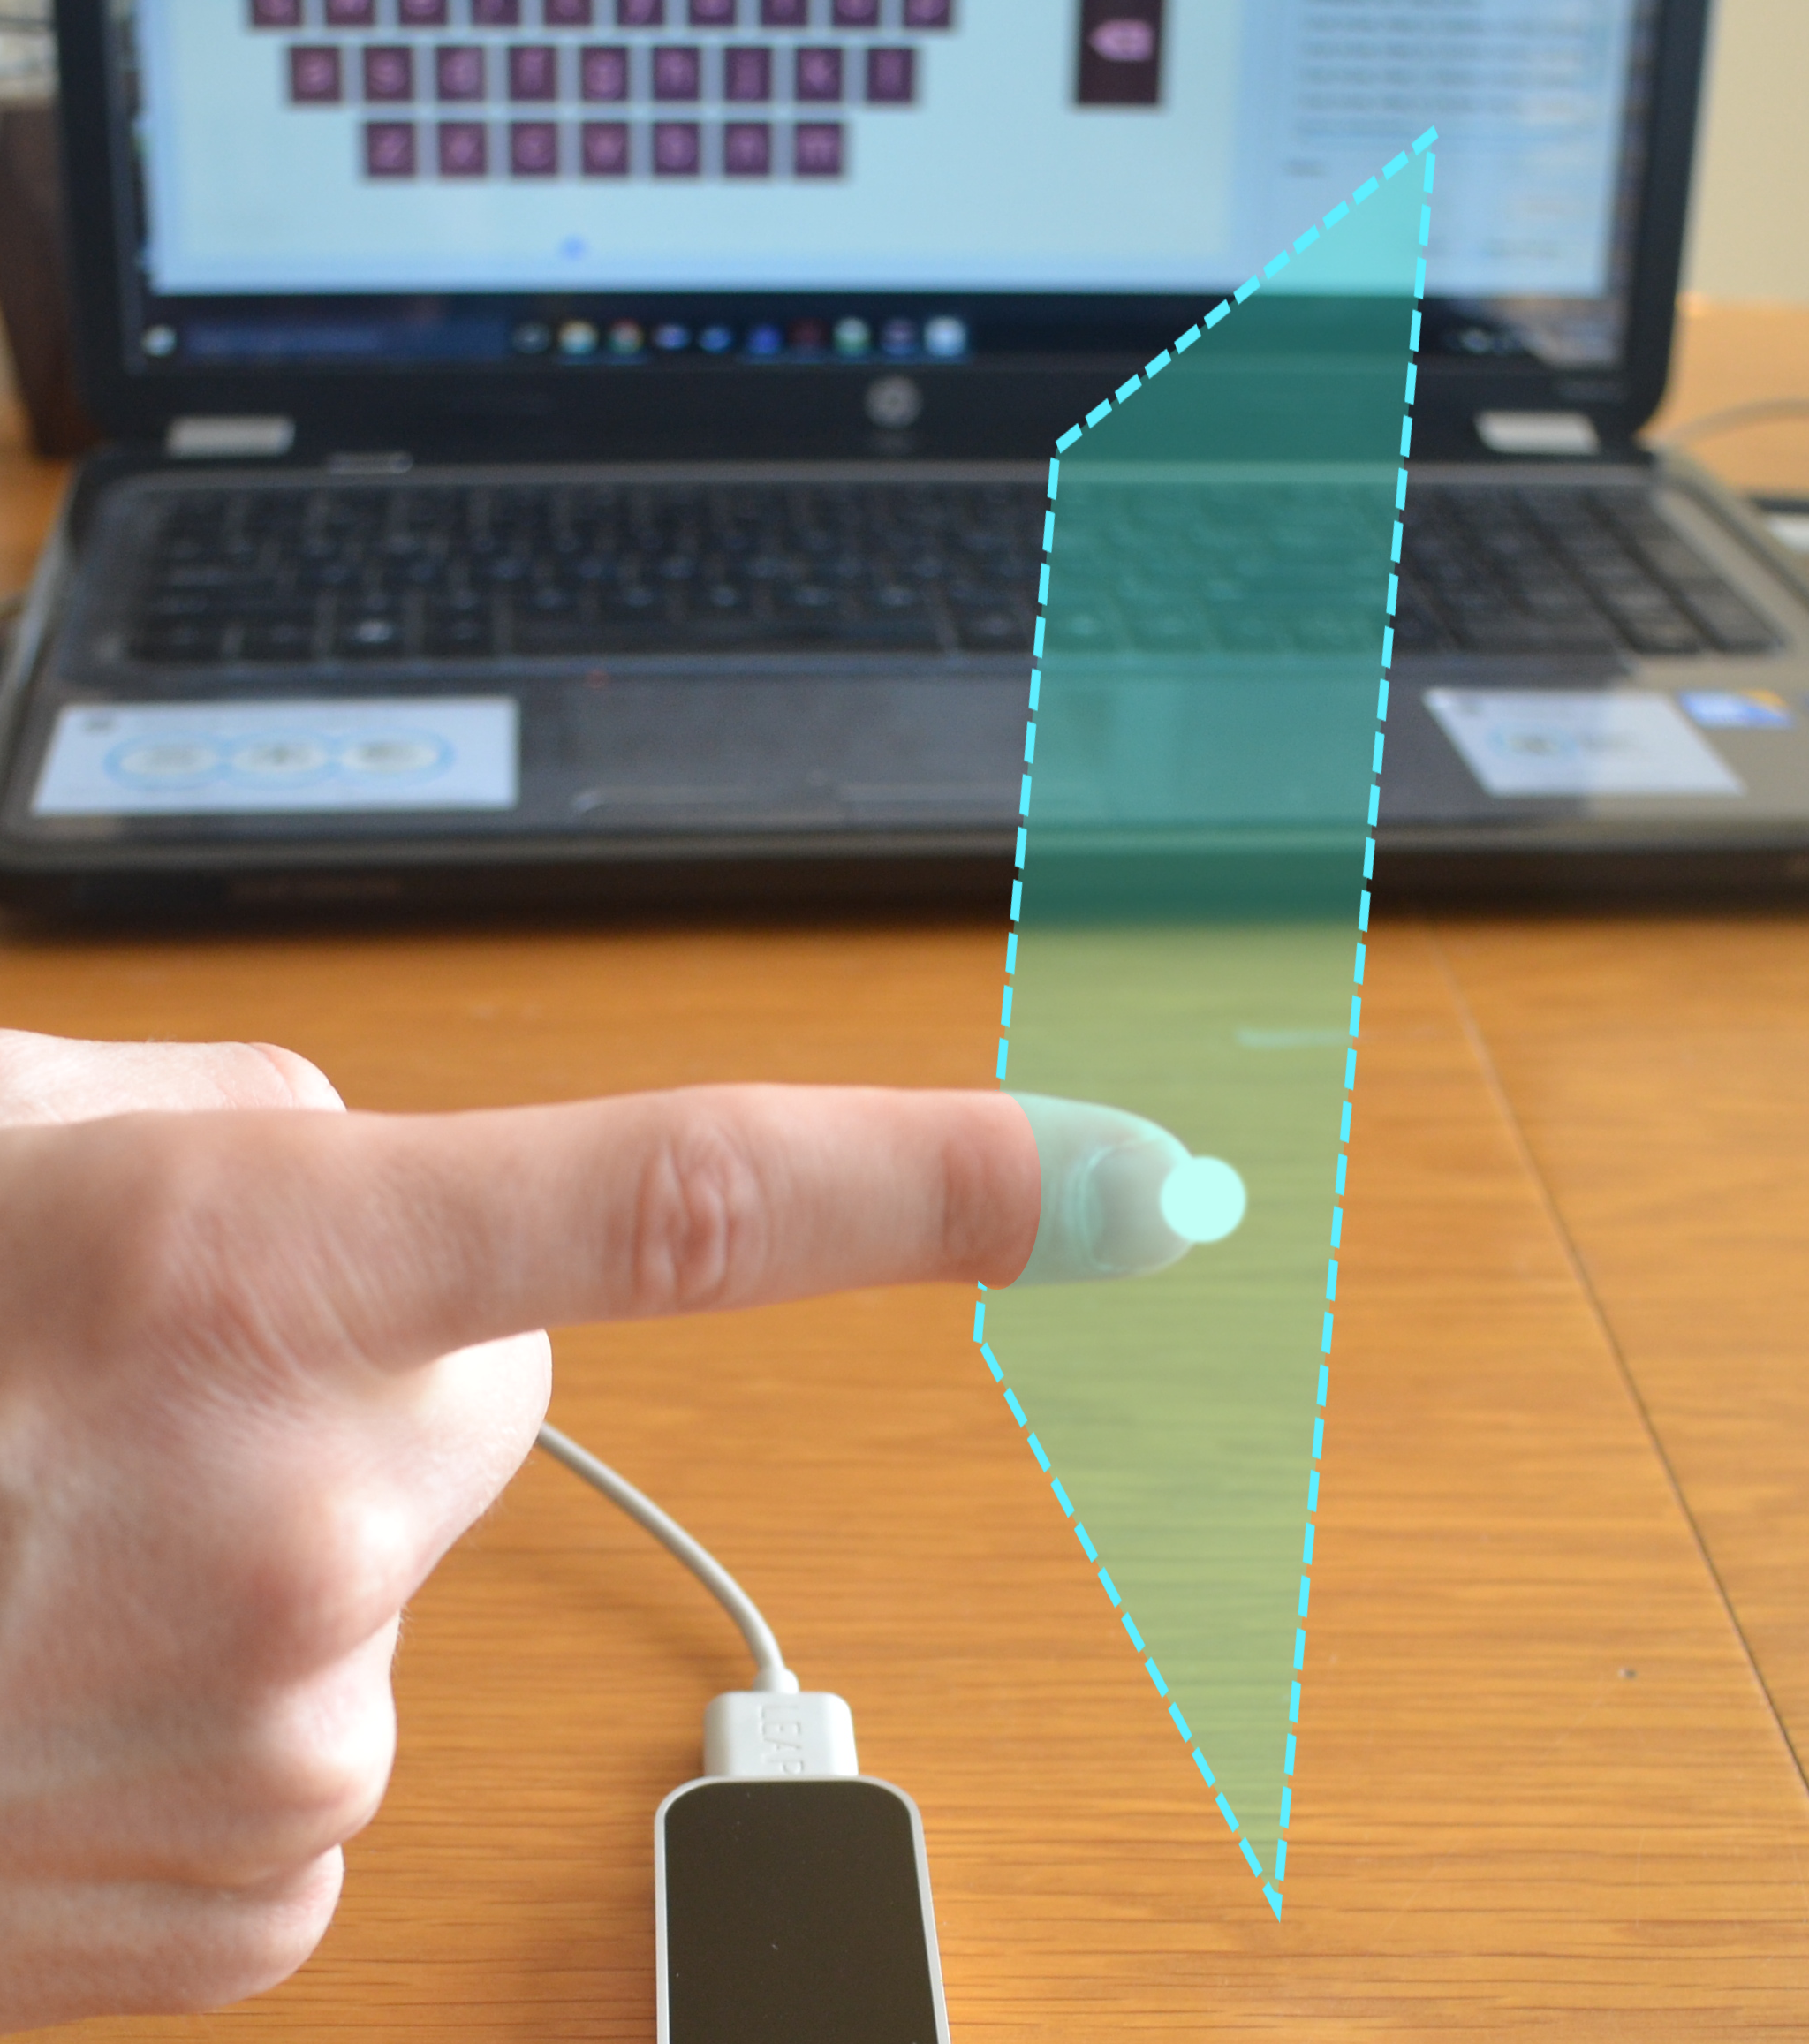
\includegraphics[width=2.5in]{fig_arc_down}
		\subcaption{Pressing Final Key}
	\end{minipage}
	\begin{minipage}[t]{2.5in}
		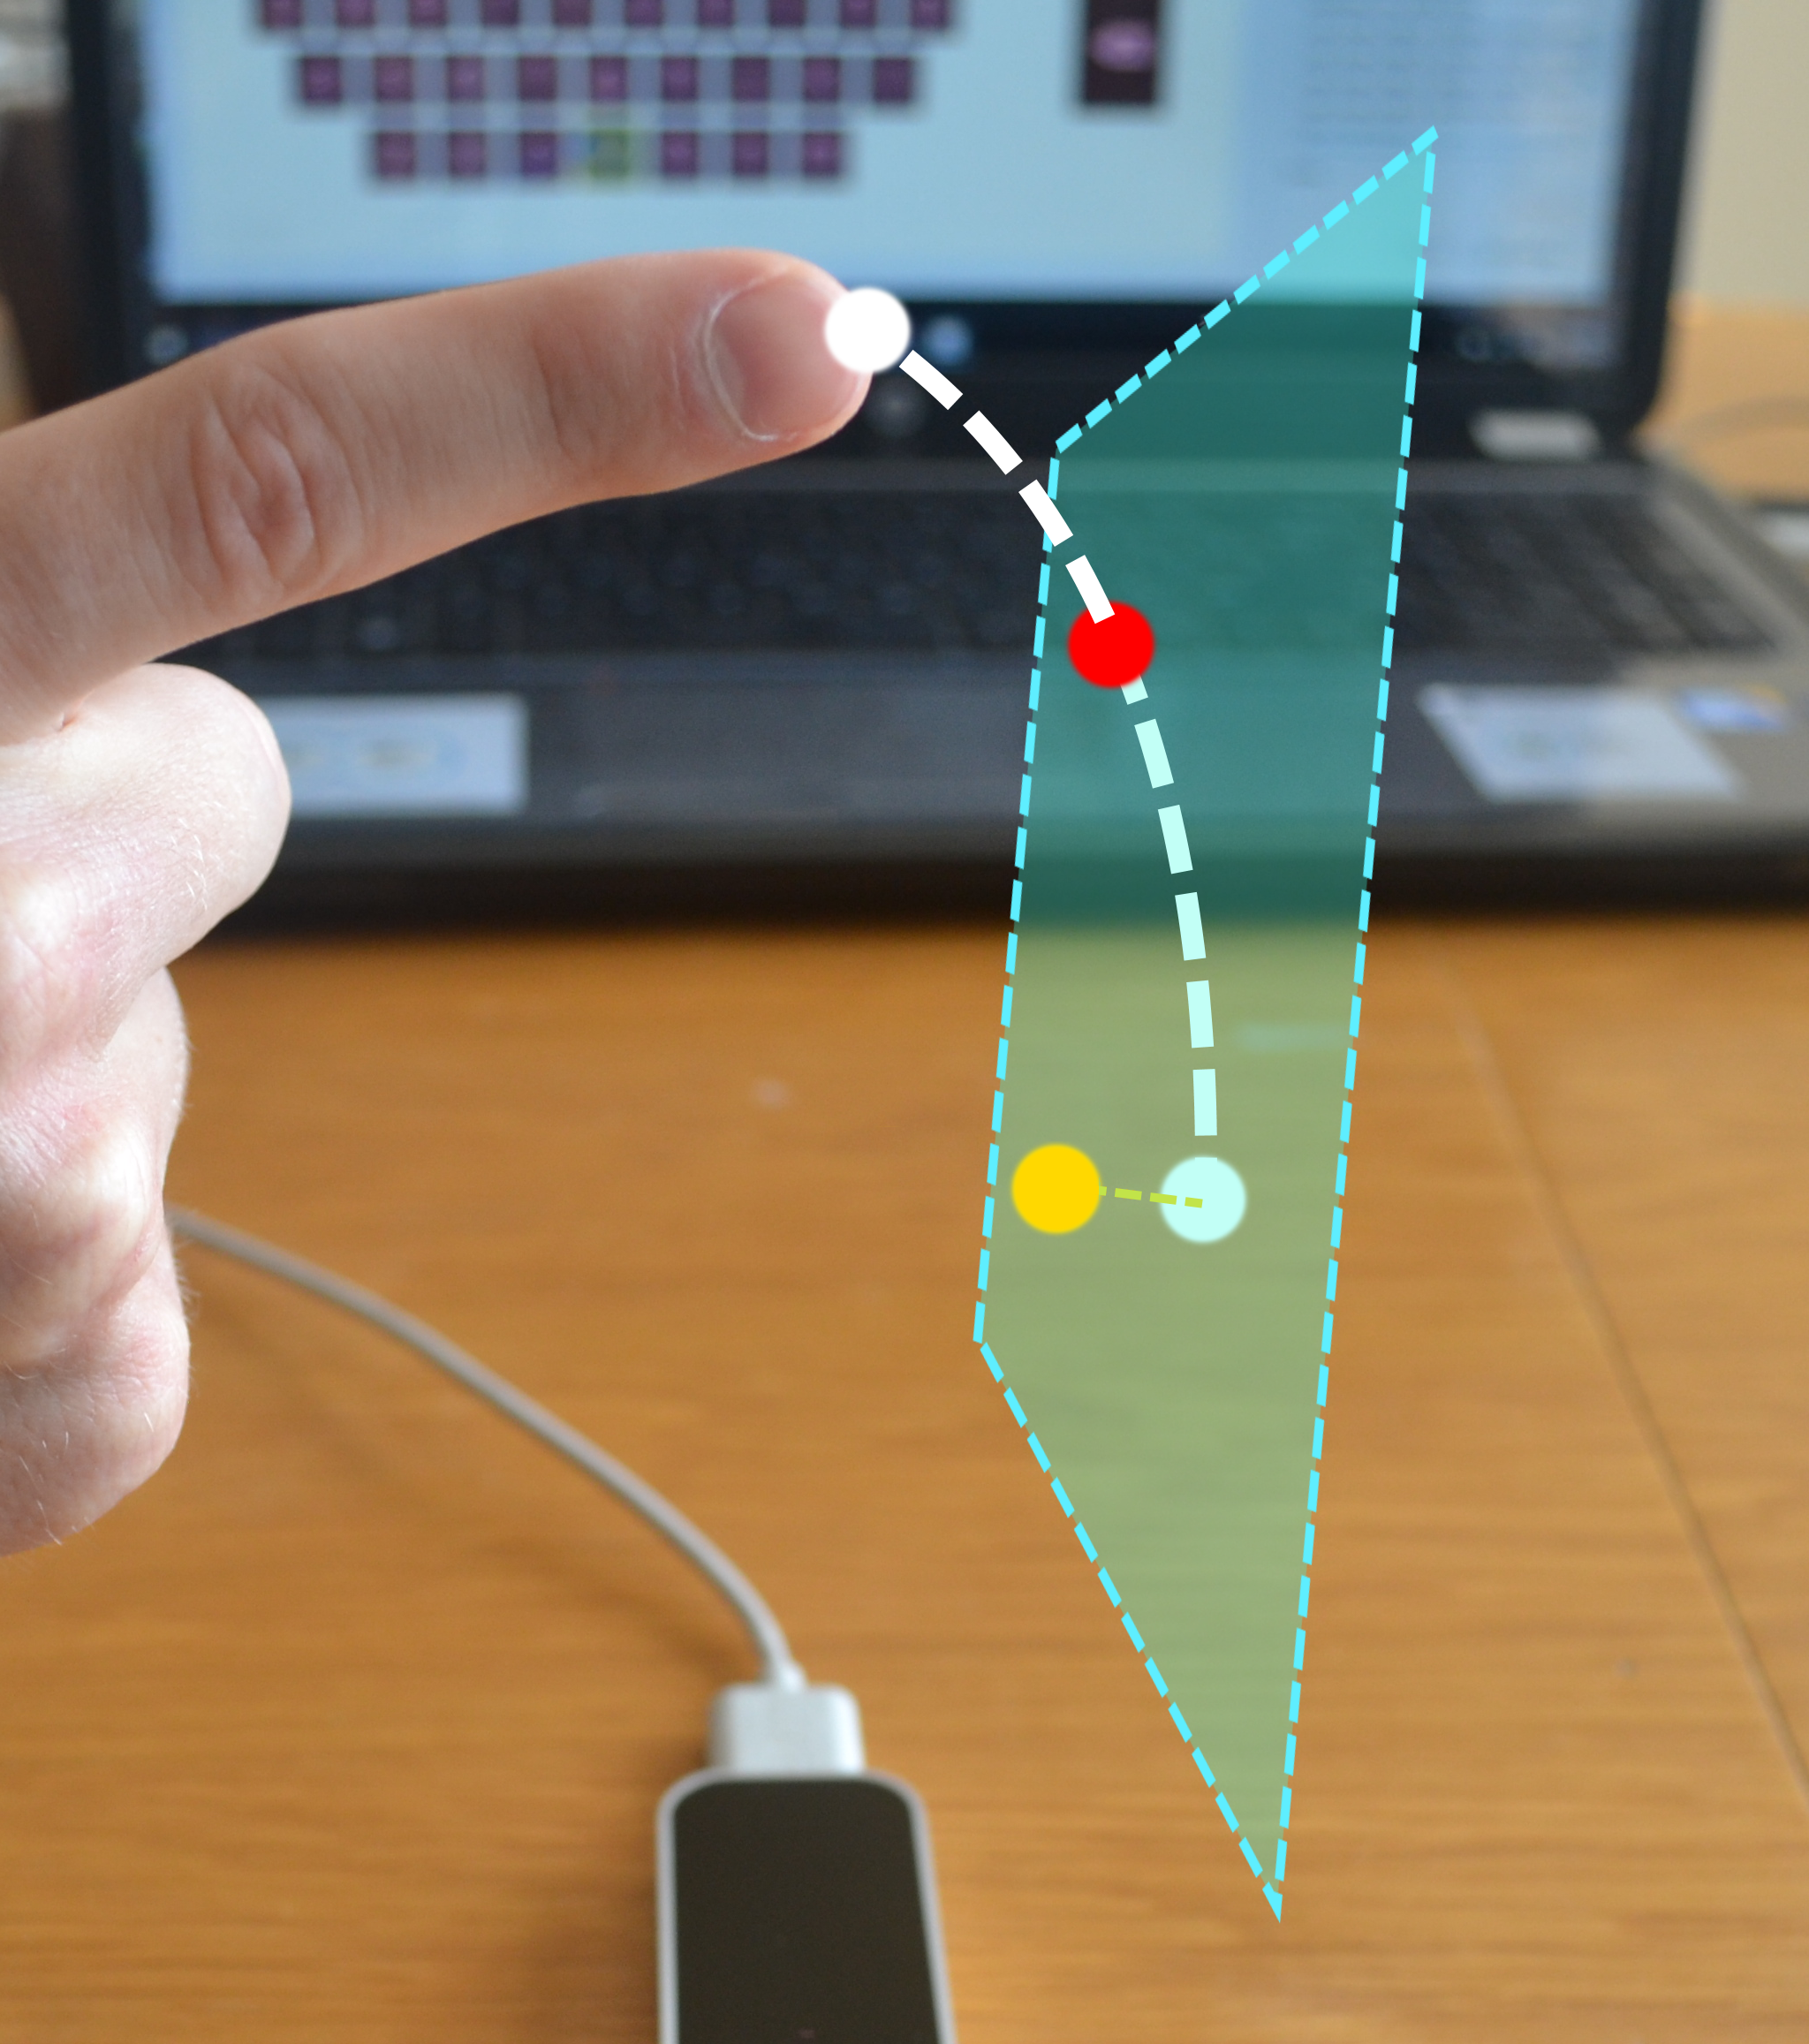
\includegraphics[width=2.5in]{fig_arc_up}
		\subcaption{Removing Hand From Plane}
	\end{minipage}
	\caption[Arcing Motion]{Examples of how the natural arcing motion generates erroneous input for 3-Dimensional interactions. \textbf{(a)} shows the user pressing the final key. \textbf{(b)} shows the intended release \textbf{yellow} and the detected release \textbf{red}.}
	\label{arcing_motion}
\end{figure}

\subsection{Keystrokes Per Character}
Figure~\ref{fig_KSPC_mean} shows the mean Keystrokes Per Character for each keyboard input device. Participants reached a mean KSPC of 1.2 keystrokes per character ($SD = 0.18$) for the Touch Screen Keyboard, 1.4 keystrokes per character  ($SD = 0.38$) for the Leap Surface Keyboard, 2.0 keystrokes per character ($SD = 0.79$) for the Leap Static-Air Keyboard, 1.6 keystrokes per character ($SD = 0.42$) for the Leap Pinch-Air Keyboard, 1.9 keystrokes per character ($SD = 0.64$) for the Predictive-Air Keyboard, and 1.2 keystrokes per character ($SD = 0.18$) for the Leap Bimodal-Air Keyboard. Using a One-Way Analysis of Variance, a significant difference was detected between keyboard means, $F(5, 102) = 9.8827$, $p$-value = 9.9960$e$-08, ($SD_{pooled} = 0.49$), prompting the use of Tukey's HSD with multiple-compare for further analysis.

\begin{figure}[h]
	\centering
	\includegraphics{fig_KSPC_mean}
	\caption[Mean Keystrokes Per Character]{Mean Keystrokes Per Character for each keyboard with error bars showing 95\% confidence intervals.}
	\label{fig_KSPC_mean}
\end{figure}

The multiple comparisons, seen in Table~\ref{KSPC_multcompare}, revealed significant differences in Keystrokes Per Character between the Touch Screen Keyboard and the Leap Static-Air and Predictive-Air keyboards, both with $p$-values $<$ 0.001. There were significant differences between the Leap Surface Keyboard and the Static-Air and Predictive-Air keyboards both with $p$-values $<$ 0.05. There were also significant differences found between the Leap Bimodal-Air and the Static-Air and Predictive-Air keyboards, both with $p$-values $<$ 0.01.

Keystrokes Per Character was useful for the pseudo, word-gesture keyboard implementation because words were constructed at the character level rather than at the word level as with word-recognition. With KSPC, if words were input without any detected errors, then we would expect a KSPC of 1.0 keystrokes. This metric helps show the rate at which extra erroneous characters were produced for each keyboard, for example, the KSPC of the Static-Air keyboard was 2.0 keystrokes, meaning 100\% more interactions were produced than required to type the words successfully. As before, the Static-Air and Predictive-Air keyboard performances were underwhelming and the Bimodal-Air performed on par with the Touch Screen and Leap Surface keyboards. The Pinch-Air performed somewhere in between the other Leap Motion-based keyboards. As could be seen, a trend was developing in the dependent measures and was expected to hold for all other variables.

\subsubsection{KSPC Modified-Shortest}
Figure~\ref{fig_KSPC_short_mean} shows the mean Keystrokes Per Character with the shortest-transcribed modification for each keyboard input device. Participants reached a mean KSPC of 1.1 keystrokes per character ($SD = 0.14$) for the Touch Screen Keyboard, 1.3 keystrokes per character ($SD = 0.27$) for the Leap Surface Keyboard, 1.7 keystrokes per character ($SD = 0.48$) for the Leap Static-Air Keyboard, 1.4 keystrokes per character ($SD = 0.31$) for the Leap Pinch-Air Keyboard, 1.7 keystrokes per character ($SD = 0.43$) for the Predictive-Air Keyboard, and 1.1 keystrokes per character ($SD = 0.15$) for the Leap Bimodal-Air Keyboard. Using a One-Way Analysis of Variance, a significant difference was detected between keyboard means, $F(5, 102) = 11.5949$, $p$-value = 7.0164$e$-09, ($SD_{pooled} = 0.32$), prompting the use of Tukey's HSD with multiple-compare for further analysis.

\begin{figure}[h]
	\centering
	\includegraphics{fig_KSPC_short_mean}
	\caption[Mean Keystrokes Per Character for Modified-Shortest]{Mean Keystrokes Per Character using the shortest-transcribed modification for each keyboard with error bars showing 95\% confidence intervals.}
	\label{fig_KSPC_short_mean}
\end{figure}

The multiple comparisons, seen in Table~\ref{KSPC_short_multcompare}, revealed significant differences in Keystrokes Per Character with the shortest-transcribed modification between the Touch Screen Keyboard and the Leap Static-Air and Predictive-Air keyboards with $p$-values $<$ 0.0001. There were significant differences between the Leap Surface Keyboard and the Leap Static-Air and Predictive-Air keyboards both with $p$-values $<$ 0.05. There were also significant differences found between the Leap Bimodal-Air and the Static-Air and Predictive-Air keyboards, both with $p$-values $<$ 0.001. Finally there was a significant difference between the Pinch-Air and Static-Air keyboards with a $p$-value = 0.0072.

As before, like with MWD, KSPC saw huge improvements with the shortest-transcribed modification, especially for Leap Motion-based keyboards. This reaffirmed that a large number of errors were produced during exiting the interaction plane.

\subsection{Minimum String Distance}

\subsubsection{MSD Modified-Shortest}
Figure~\ref{fig_MSD_short_mean} shows the mean Minimum String Distance with the shortest-transcribed modification for each keyboard input device. Participants reached a mean MSD of 1.6\% ($SD = 2.4$) for the Touch Screen Keyboard, 2.2\% ($SD = 2.4$) for the Leap Surface Keyboard, 6.4\% ($SD = 5.0$) for the Leap Static-Air Keyboard, 5.1\% ($SD = 3.1$) for the Leap Pinch-Air Keyboard, 5.4\% ($SD = 3.3$) for the Predictive-Air Keyboard, and 2.5\% ($SD = 2.6$) for the Leap Bimodal-Air Keyboard. Using a One-Way Analysis of Variance, a significant difference was detected between keyboard means, $F(5, 102) = 6.8688$, $p$-value = 1.4591$e$-05, ($SD_{pooled} = 3.3$), prompting the use of Tukey's HSD with multiple-compare for further analysis.

\begin{figure}[h]
	\centering
	\includegraphics{fig_MSD_short_mean}
	\caption[Mean Minimum String Distance for Modified-Shortest]{Mean Minimum String Distance using the shortest-transcribed modification for each keyboard with error bars showing 95\% confidence intervals.}
	\label{fig_MSD_short_mean}
\end{figure}

The multiple comparisons, seen in Table~\ref{MSD_short_multcompare}, revealed significant differences in Minimum String Distance with the shortest-transcribed modification between the Touch Screen Keyboard and the Leap Static-Air, Pinch-Air, and Predictive-Air keyboards with $p$-values $<$ 0.05. There were significant differences between the Leap Surface Keyboard and the Leap Static-Air and Predictive-Air keyboards both with $p$-values $<$ 0.05. There were also significant differences found between the Leap Bimodal-Air and the Static-Air keyboards with a $p$-value $=$ 0.0067.

The error rates seen for the Pinch-Air and Touch Screen keyboards for MSD with the shortest-transcribed modification were similar to those found in Vulture for their MWD \cite{ref_vulture}. It is expected that with practice or repeated sessions, these error rates would become even less. The keyboards again follow the same pattern as other measures, providing more evidence of the effects of decoupling on performance and complexity of 3-Dimensions versus a physical surface. Notably, the Leap Bimodal-Air seems to be mostly unaffected by decoupling between the motor space and display space and seems to be only minimally affected by complexity, so far having never been significantly different than the Touch Screen or the Leap Surface keyboards.

\subsection{Total Error Rate}
Figure~\ref{fig_totER_mean} shows the mean Total Error Rate for each keyboard input device. Participants reached a mean Total Error Rate of 4.9\% ($SD = 5.5$) for the Touch Screen Keyboard, 9.3\% ($SD = 7.1$) for the Leap Surface Keyboard, 23.6\% ($SD = 12.1$) for the Leap Static-Air Keyboard, 14.1\% ($SD = 9.0$) for the Leap Pinch-Air Keyboard, 20.1\% ($SD = 11.4$) for the Predictive-Air Keyboard, and 6.8\% ($SD = 5.5$) for the Leap Bimodal-Air Keyboard. Using a One-Way Analysis of Variance, a significant difference was detected between keyboard means, $F(5, 102) = 12.9381$, $p$-value = 9.4983$e$-10, ($SD_{pooled} = 8.8$), prompting the use of Tukey's HSD with multiple-compare for further analysis.

\begin{figure}[h]
	\centering
	\includegraphics{fig_totER_mean}
	\caption[Mean Total Error Rates]{Mean Total Error Rates for each keyboard with error bars showing 95\% confidence intervals.}
	\label{fig_totER_mean}
\end{figure}

The multiple comparisons, seen in Table~\ref{totER_multcompare}, revealed significant differences in Total Error Rate between the Touch Screen Keyboard and the Leap Static-Air and Predictive-Air keyboards, both with $p$-values $<$ 0.0001. There were significant differences between the Leap Surface Keyboard and the Static-Air and Predictive-Air keyboards both with $p$-values $<$ 0.01. There were also significant differences found between the Leap Bimodal-Air and the Static-Air and Predictive-Air keyboards, both with $p$-values $<$ 0.01. Finally, there was a significant difference between the Pinch-Air and the Static-Air keyboards with a $p$-value = 0.0191.

Again, we see the keyboards following the same pattern. The Bimodal-Air and Leap Surface keyboards perform about as well as the Touch Screen Keyboard while the Static-Air and Predictive-Air keyboards continue to fall short. The Pinch-Air keyboard falls somewhere in the middle for Total Error Rate, not significantly different from any of them.

\subsubsection{Total Error Rate Modified-Shortest}
Figure~\ref{fig_totER_short_mean} shows the mean Total Error Rate with the shortest-transcribed modification for each keyboard input device. Participants reached a mean Total Error Rate of 4.9\% ($SD = 5.4$) for the Touch Screen Keyboard, 9.2\% ($SD = 7.0$) for the Leap Surface Keyboard, 23.3\% ($SD = 11.8$) for the Leap Static-Air Keyboard, 13.5\% ($SD = 8.9$) for the Leap Pinch-Air Keyboard, 19.4\% ($SD = 10.7$) for the Predictive-Air Keyboard, and 6.7\% ($SD = 5.3$) for the Leap Bimodal-Air Keyboard. Using a One-Way Analysis of Variance, a significant difference was detected between keyboard means, $F(5, 102) = 13.0717$, $p$-value = 7.8147$e$-10, ($SD_{pooled} = 8.6$), prompting the use of Tukey's HSD with multiple-compare for further analysis.

\begin{figure}[h]
	\centering
	\includegraphics{fig_totER_short_mean}
	\caption[Mean Total Error Rate for Modified-Shortest]{Mean Total Error Rate using the shortest-transcribed modification for each keyboard with error bars showing 95\% confidence intervals.}
	\label{fig_totER_short_mean}
\end{figure}

The multiple comparisons, seen in Table~\ref{totER_short_multcompare}, revealed significant differences in Total Error Rate with the shortest-transcribed modification between the Touch Screen Keyboard and the Leap Static-Air, Pinch-Air, and Predictive-Air keyboards with $p$-values $<$ 0.05. There were significant differences between the Leap Surface Keyboard and the Leap Static-Air and Predictive-Air keyboards both with $p$-values $<$ 0.01. There were also significant differences found between the Leap Bimodal-Air and the Static-Air and Predictive-Air keyboards with a $p$-value $<$ 0.001. Finally, there was a significant difference between the Pinch-Air and Static-Air keyboards with a $p$-value = 0.0101.

Surprisingly, unlike KSPC and MWD, the Total Error Rate did not follow suit and show large decreases in error rate with the shortest-transcribed modification; however, these observations still support what was seen with text-entry rates also being relatively unaffected by the shortest-transcribed modification. This further implied that errors made by participants were more likely corrected throughout typing the words rather than at the end. This was a major downside of lacking word-recognition because gestures were interrupted and corrected rather than being followed through completely as is natural with word-gesture keyboards.

\section{Correctness}

\subsection{Fr\'echet Distance} \label{results_frechet}
Figure~\ref{fig_frechet_mean} shows the mean Fr\'echet Distance for each keyboard input device. Participants reached a mean Fr\'echet Distance of 231.2 pixels ($SD = 26.7$) for the Touch Screen Keyboard, 242.8 pixels ($SD = 30.4$) for the Leap Surface Keyboard, 364.3 pixels ($SD = 86.5$) for the Leap Static-Air Keyboard, 501.2 pixels ($SD = 42.8$) for the Leap Pinch-Air Keyboard, 350.6 pixels ($SD = 86.8$) for the Predictive-Air Keyboard, and 396.5 pixels ($SD = 102.1$) for the Leap Bimodal-Air Keyboard. Using a One-Way Analysis of Variance, a significant difference was detected between keyboard means, $F(5, 102) = 37.9416$, $p$-value = 8.0562$e$-22, ($SD_{pooled} = 69.4$), prompting the use of Tukey's HSD with multiple-compare for further analysis.

\begin{figure}[h]
	\centering
	\includegraphics{fig_frechet_mean}
	\caption[Mean Fr\'echet Distance]{Mean Fr\'echet Distance for each keyboard with error bars showing 95\% confidence intervals.}
	\label{fig_frechet_mean}
\end{figure}

The multiple comparisons, seen in Table~\ref{frechet_multcompare}, revealed significant differences in Fr\'echet Distance between the Touch Screen Keyboard and all of the mid-air keyboards with $p$-values $<$ 0.0001. There were significant differences between the Leap Surface Keyboard and all of the mid-air keyboards with $p$-values $<$ 0.001. There were also significant differences found between the Leap Pinch-Air and all of the other mid-air keyboards with $p$-values $<$ 0.001.

The Fr\'echet Distance was the only place where the trends were broken and the Bimodal-Air keyboard performs significantly worse than the Touch Screen and Leap Surface keyboards. The Pinch-Air Keyboard also performed significantly worse than all other keyboards. These results are expected to be caused by a combination of the word-gesture velocity seen in Section~\ref{results_velocity_gesture} and the affects of increase decoupling or complexity from working with the 3rd-Dimension.

The Leap Bimodal-Air seemed to suffer in correctness due to its very high word-gesture velocities whereas the Static-Air and Predictive-Air benefit in correctness due to their very slow word-gesture velocities. The Leap Surface and Touch Screen keyboards were relatively unaffected in correctness by their high word-gesturing velocities due to their decreased decoupling from the word-gesture motor space to the displayed screen. 

The Pinch-Air Keyboard suffered from the combination of high word-gesture velocities and effects of increased decoupling; however, it also seems to be affected heavily by it's deviation in its tracking method increasing its overall distance traveled for each word-gesture, see Section~\ref{results_distance}. All other mid-air keyboards track the participant's pointer finger whereas the Pinch-Air keyboard tracks the participant's palm since their fingers move so sharply when creating a pinching gesture. This difference in tracking combined with high word-gesture velocities are the expected factors for this decrease in performance.

\subsubsection{Fr\'echet Distance Modified-Shortest}
Figure~\ref{fig_frechet_short_mean} shows the mean Fr\'echet Distance with the shortest-transcribed modification for each keyboard input device. Participants reached a mean Fr\'echet Distance of 221.0 pixels ($SD = 18.0$) for the Touch Screen Keyboard, 231.0 pixels ($SD = 22.7$) for the Leap Surface Keyboard, 306.4 pixels ($SD = 53.2$) for the Leap Static-Air Keyboard, 459.2 pixels ($SD = 20.1$) for the Leap Pinch-Air Keyboard, 281.6 pixels ($SD = 49.9$) for the Predictive-Air Keyboard, and 368.4 pixels ($SD = 82.4$) for the Leap Bimodal-Air Keyboard. Using a One-Way Analysis of Variance, a significant difference was detected between keyboard means, $F(5, 102) = 65.7440$, $p$-value = 2.3767$e$-30, ($SD_{pooled} = 47.2$), prompting the use of Tukey's HSD with multiple-compare for further analysis.

\begin{figure}[h]
	\centering
	\includegraphics{fig_frechet_short_mean}
	\caption[Mean Fr\'echet Distance for Modified-Shortest]{Mean Fr\'echet Distance using the shortest-transcribed modification for each keyboard with error bars showing 95\% confidence intervals.}
	\label{fig_frechet_short_mean}
\end{figure}

The multiple comparisons, seen in Table~\ref{frechet_short_multcompare}, revealed significant differences in Fr\'echet Distance with the shortest-transcribed modification between the Touch Screen Keyboard and all of the mid-air keyboards with $p$-values $<$ 0.01. There were significant differences between the Leap Surface Keyboard and all of the mid-air keyboards with $p$-values $<$ 0.05. There were also significant differences found between the Leap Bimodal-Air Keyboard and the other mid-air keyboards with $p$-values $<$ 0.01. Finally, there were significant differences found between the Leap Pinch-Air Keyboard and the Static-Air and Predictive-Air keyboards with $p$-values $<$ 0.0001.

Again, the increase in correctness for all keyboards, namely the mid-air keyboards, when using the shortest-transcribed modification implies that many errors were being produced when exiting the interaction plane. This was especially evident for the Static-Air, Pinch-Air, and Predictive-Air keyboards all seeing the largest improvements. For the Static-Air and Predictive-Air keyboards, these errors were caused by the addition of the 3rd-Dimension and participants having trouble entering and exiting the interaction plane accurately. The Pinch-Air Keyboard, again, sees a combination of high word-gesture velocity and a difference in tracking that was expected to produce these kinds of errors.

\subsubsection{Fr\'echet Distance Modified-Backspace}
Figure~\ref{fig_frechet_back_mean} shows the mean Fr\'echet Distance with the backspace-transcribed modification for each keyboard input device. Participants reached a mean Fr\'echet Distance of 212.3 pixels ($SD = 9.3$) for the Touch Screen Keyboard, 223.5 pixels ($SD = 18.5$) for the Leap Surface Keyboard, 258.9 pixels ($SD = 33.5$) for the Leap Static-Air Keyboard, 444.7 pixels ($SD = 8.0$) for the Leap Pinch-Air Keyboard, 237.7 pixels ($SD = 24.8$) for the Predictive-Air Keyboard, and 356.8 pixels ($SD = 85.0$) for the Leap Bimodal-Air Keyboard. Using a One-Way Analysis of Variance, a significant difference was detected between keyboard means, $F(5, 102) = 97.1196$, $p$-value = 3.5271$e$-37, ($SD_{pooled} = 39.7$), prompting the use of Tukey's HSD with multiple-compare for further analysis.

\begin{figure}[h]
	\centering
	\includegraphics{fig_frechet_back_mean}
	\caption[Mean Fr\'echet Distance for Modified-Backspace]{Mean Fr\'echet Distance using the backspace-transcribed modification for each keyboard with error bars showing 95\% confidence intervals.}
	\label{fig_frechet_back_mean}
\end{figure}

The multiple comparisons, seen in Table~\ref{frechet_back_multcompare}, revealed significant differences in Fr\'echet Distance with the backspace-transcribed modification between the Touch Screen Keyboard and the Leap Static-Air, Pinch-Air, and Bimodal-Air keyboards with $p$-values $<$ 0.01. There were significant differences between the Leap Surface Keyboard and the Leap Pinch-Air and Bimodal-Air keyboards both with $p$-values $<$ 0.0001. There were also significant differences found between the Leap Bimodal-Air and all other mid-air keyboards with $p$-values $<$ 0.0001. Finally, there were significant differences between the Leap Pinch-Air Keyboard and the Static-Air and Predictive-Air keyboards with $p$-values $<$ 0.0001.

If the backspace key was included in the path considered to be correct for Fr\'echet Distance, since participants were required to correct words, a boost in correctness was observed. The Bimodal-Air and Pinch-Air keyboards still suffer from the previously mentioned problems in Section~\ref{results_frechet}. The Static-Air and Predictive-Air, however, see huge improvements in correctness because of the low word-gesture velocities and high error rates. The Predictive-Air Keyboard, in this case, was not significantly different than the Touch Screen and Leap Surface keyboards, implying that participants were relatively attentive to correcting errors for it.

\section{Distance Measures}
\subsection{Word-Gesture Distance} \label{results_distance}
Figure~\ref{fig_distance_mean} shows the mean Word-Gesture Distance for each keyboard input device. Participants reached a mean Word-Gesture Distance of 1087.5 pixels ($SD = 85.9$) for the Touch Screen Keyboard, 1423.9 pixels ($SD = 246.0$) for the Leap Surface Keyboard, 1590.9 pixels ($SD = 508.2$) for the Leap Static-Air Keyboard, 2165.3 pixels ($SD = 540.5$) for the Leap Pinch-Air Keyboard, 1634.7 pixels ($SD = 481.4$) for the Predictive-Air Keyboard, and 1627.7 pixels ($SD = 321.3$) for the Leap Bimodal-Air Keyboard. Using a One-Way Analysis of Variance, a significant difference was detected between keyboard means, $F(5, 102) = 13.9225$, $p$-value = 2.2937$e$-10, ($SD_{pooled} = 398.6$), prompting the use of Tukey's HSD with multiple-compare for further analysis.

\begin{figure}[h]
	\centering
	\includegraphics{fig_distance_mean}
	\caption[Mean Word-Gesture Distance]{Mean Word-Gesture Distance for each keyboard with error bars showing 95\% confidence intervals.}
	\label{fig_distance_mean}
\end{figure}

The multiple comparisons, seen in Table~\ref{distance_multcompare}, revealed significant differences in Word-Gesture Distance between the Touch Screen Keyboard and all of the mid-air keyboards with $p$-values $<$ 0.01. There was a significant difference between the Leap Pinch-Air and all other Leap Motion keyboards with $p$-values $<$ 0.01.

As expected, all mid-air keyboards required longer word-gesture distances than the Touch Screen Keyboard due to the effect of decoupling between the word-gesture motor space and the keyboard display. It was surprising, however, that the Leap Surface Keyboard had required significantly more word-gesture distance than the Touch Screen Keyboard. This could be because of the requirement to use a stylus rather than the participants bare hand.

The Pinch-Air keyboard required a significantly longer word-gesture distance than all other keyboards. This was expected to be caused by the difference in tracking method as previously mentioned. Tracking the palm requires larger, less controlled movements than with tracking fingers or a stylus.

\subsubsection{Word-Gesture Distance Modified-Shortest}
Figure~\ref{fig_distance_short_mean} shows the mean Word-Gesture Distance with the shortest-transcribed modification for each keyboard input device. Participants reached a mean Word-Gesture Distance of 1081.3 ($SD = 84.6$) for the Touch Screen Keyboard, 1396.5 ($SD = 226.5$) for the Leap Surface Keyboard, 1524.8 ($SD = 412.5$) for the Leap Static-Air Keyboard, 1981.4 ($SD = 470.6$) for the Leap Pinch-Air Keyboard, 1536.7 ($SD = 346.1$) for the Predictive-Air Keyboard, and 1566.5 ($SD = 253.6$) for the Leap Bimodal-Air Keyboard. Using a One-Way Analysis of Variance, a significant difference was detected between keyboard means, $F(5, 102) = 14.403$, $p$-value = 1.1613$e$-10, ($SD_{pooled} = 325.1$), prompting the use of Tukey's HSD with multiple-compare for further analysis.

\begin{figure}[h]
	\centering
	\includegraphics{fig_distance_short_mean}
	\caption[Mean Word-Gesture Distance for Modified-Shortest]{Mean Word-Gesture Distance using the shortest-transcribed modification for each keyboard with error bars showing 95\% confidence intervals.}
	\label{fig_distance_short_mean}
\end{figure}

The multiple comparisons, seen in Table~\ref{distance_short_multcompare}, revealed significant differences in Word-Gesture Distance with the shortest-transcribed modification between the Touch Screen Keyboard and all other keyboards with $p$-values $<$ 0.05. There were significant differences between the Leap Surface and Pinch-Air keyboards and all other Leap Motion keyboards with $p$-values $<$ 0.01.

Again, the small difference between the word-gesture distance and the word-gesture distance using the shortest-transcribed modification, implies that most errors were corrected by participants whilst in the middle of typing words.

\subsection{Word-Gesture Velocity} \label{results_velocity_gesture}
Figure~\ref{fig_velocity_gesture_mean} shows the mean Word-Gesture Velocity for each keyboard input device. Participants reached a mean Word-Gesture Velocity of 673.3 $pixels/s$ ($SD = 126.4$) for the Touch Screen Keyboard, 641.1 $pixels/s$ ($SD = 165.5$) for the Leap Surface Keyboard, 380.9 $pixels/s$ ($SD = 78.2$) for the Leap Static-Air Keyboard, 643.8 $pixels/s$ ($SD = 204.7$) for the Leap Pinch-Air Keyboard, 405.6 $pixels/s$ ($SD = 87.6$) for the Predictive-Air Keyboard, and 777.6 $pixels/s$ ($SD = 240.9$) for the Leap Bimodal-Air Keyboard. Using a One-Way Analysis of Variance, a significant difference was detected between keyboard means, $F(5, 102) = 17.233$, $p$-value = 2.4922$e$-12, ($SD_{pooled} = 161.8$), prompting the use of Tukey's HSD with multiple-compare for further analysis.

\begin{figure}[h]
	\centering
	\includegraphics{fig_velocity_gesture_mean}
	\caption[Mean Word-Gesture Velocity]{Mean Word-Gesture Velocity for each keyboard with error bars showing 95\% confidence intervals.}
	\label{fig_velocity_gesture_mean}
\end{figure}

The multiple comparisons, seen in Table~\ref{velocity_gesture_multcompare}, revealed significant differences in Word-Gesture Velocity between the Touch Screen Keyboard and the Leap Static-Air and Predictive-Air keyboards with $p$-values $<$ 0.0001. There were significant differences between the Leap Surface Keyboard and the Static-Air and Predictive-Air keyboards with $p$-values $<$ 0.001. There were also significant differences found between the Leap Bimodal-Air and the Static-Air and Predictive-Air keyboards with $p$-values $<$ 0.0001. Finally, there were significant differences found between the Leap Pinch-Air and the Static-Air and Predictive Air keyboards with $p$-values $<$ 0.001.

The Static-Air and Predictive-Air keyboards were significantly slower than all of the other keyboards for word-gesture velocity. This was expected due to the enhanced precision required when working with a 3rd-Dimension in mid-air. It is interesting that these two keyboards also had the highest error rates across all error measures, implying a very high degree of difficulty, even with slower movements.

\subsection{Hand Velocity}
Figure~\ref{fig_velocity_hand_mean} shows the mean Hand Velocity for each keyboard input device. Participants reached a mean Hand Velocity of 35.7 $cm/s$ ($SD = 6.7$) for the Touch Screen Keyboard, 15.0 $cm/s$ ($SD = 3.9$) for the Leap Surface Keyboard, 6.9 $cm/s$ ($SD = 1.4$) for the Leap Static-Air Keyboard, 10.5 $cm/s$ ($SD = 3.2$) for the Leap Pinch-Air Keyboard, 7.6 $cm/s$ ($SD = 1.7$) for the Predictive-Air Keyboard, and 15.2 $cm/s$ ($SD = 5.1$) for the Leap Bimodal-Air Keyboard. Using a One-Way Analysis of Variance, a significant difference was detected between keyboard means, $F(5, 102) = 121.9826$, $p$-value = 2.0877$e$-41, ($SD_{pooled} = 4.1$), prompting the use of Tukey's HSD with multiple-compare for further analysis.

\begin{figure}[h]
	\centering
	\includegraphics{fig_velocity_hand_mean}
	\caption[Mean Hand Velocity]{Mean Hand Velocity for each keyboard with error bars showing 95\% confidence intervals.}
	\label{fig_velocity_hand_mean}
\end{figure}

The multiple comparisons, seen in Table~\ref{velocity_hand_multcompare}, revealed significant differences in Hand Velocity between the Touch Screen Keyboard and all other keyboards with $p$-values $<$ 0.0001. There were significant differences between the Leap Surface Keyboard and the Static-Air, Pinch-Air, and Predictive-Air keyboards with $p$-values $<$ 0.05. There were also significant differences found between the Leap Bimodal-Air and all other mid-air keyboards with $p$-values $<$ 0.05.

The hand velocities were all similar to the word-gesture velocities in Section~\ref{results_velocity_gesture}, except for the Touch Screen Keyboard. This result was simply caused by the difference in physical size between the interaction planes that participants used and the size of the Touch Screen used, as mentioned in Chapter~\ref{keyboard_design}.

\section{Timing Measures}

\subsection{Word-Gesture Duration}
Figure~\ref{fig_time_mean} shows the mean Word-Gesture Duration for each keyboard input device. Participants reached a mean Word-Gesture Duration of 1.65 $s$ ($SD = 0.46$) for the Touch Screen Keyboard, 2.03 $s$ ($SD = 1.17$) for the Leap Surface Keyboard, 4.01 $s$ ($SD = 1.17$) for the Leap Static-Air Keyboard, 3.36 $s$ ($SD = 0.76$) for the Leap Pinch-Air Keyboard, 3.87 $s$ ($SD = 1.18$) for the Predictive-Air Keyboard, and 2.18 $s$ ($SD = 0.36$) for the Leap Bimodal-Air Keyboard. Using a One-Way Analysis of Variance, a significant difference was detected between keyboard means, $F(5, 102) = 28.1205$, $p$-value = 8.2440$e$-18, ($SD_{pooled} = 0.81$), prompting the use of Tukey's HSD with multiple-compare for further analysis.

\begin{figure}[h]
	\centering
	\includegraphics{fig_time_mean}
	\caption[Mean Word-Gesture Duration]{Mean Word-Gesture Duration for each keyboard with error bars showing 95\% confidence intervals.}
	\label{fig_time_mean}
\end{figure}

The multiple comparisons, seen in Table~\ref{time_multcompare}, revealed significant differences in Word-Gesture Duration between the Touch Screen Keyboard and the Leap Static-Air, Pinch-Air, and Predictive-Air keyboards, all with $p$-values $<$ 0.0001. There were significant differences between the Leap Surface Keyboard and the Static-Air, Pinch-Air, and Predictive-Air keyboards, all with $p$-values $<$ 0.001. There were also significant differences found between the Leap Bimodal-Air and all of the other mid-air keyboards with $p$-values $<$ 0.001.

As expected, the Static-Air, Pinch-Air, and Predictive-Air keyboards had significantly longer word-gesture durations than the other keyboards. For the Static-Air and Predictive-Air, lower velocities and higher decoupling mean that word-gestures take longer to perform, whereas for the Pinch-Air Keyboard, the longer distances traveled were the influence for the longer durations. The Bimodal-Air keyboard performed as well as the Touch Screen and Leap Surface keyboards as expected from it's prior trends. 

\subsubsection{Word-Gesture Duration Modified-Shortest}
Figure~\ref{fig_time_short_mean} shows the mean Word-Gesture Duration with the shortest-transcribed modification for each keyboard input device. Participants reached a mean Word-Gesture Duration of 1.60 $s$ ($SD = 0.40$) for the Touch Screen Keyboard, 2.00 $s$ ($SD = 0.55$) for the Leap Surface Keyboard, 3.75 $s$ ($SD = 0.93$) for the Leap Static-Air Keyboard, 3.17 $s$ ($SD = 0.73$) for the Leap Pinch-Air Keyboard, 3.56 $s$ ($SD = 0.86$) for the Predictive-Air Keyboard, and 2.16 $s$ ($SD = 0.36$) for the Leap Bimodal-Air Keyboard. Using a One-Way Analysis of Variance, a significant difference was detected between keyboard means, $F(5, 102) = 32.0355$, $p$-value = 1.7009$e$-19, ($SD_{pooled} = 0.67$), prompting the use of Tukey's HSD with multiple-compare for further analysis.

\begin{figure}[h]
	\centering
	\includegraphics{fig_time_short_mean}
	\caption[Mean Word-Gesture Duration for Modified-Shortest]{Mean Word-Gesture Dur using the shortest-transcribed modification for each keyboard with error bars showing 95\% confidence intervals.}
	\label{fig_time_short_mean}
\end{figure}

The multiple comparisons, seen in Table~\ref{time_short_multcompare}, revealed significant differences in Word-Gesture Duration with the shortest-transcribed modification between the Touch Screen Keyboard and the Leap Static-Air, Pinch-Air, and Predictive-Air keyboards with $p$-values $<$ 0.0001. There were significant differences between the Leap Surface Keyboard and the Leap Static-Air, Pinch-Air, and Predictive-Air keyboards all with $p$-values $<$ 0.0001. There were also significant differences found between the Leap Bimodal-Air and all of the other mid-air keyboards with $p$-values $<$ 0.001.

As seen before, the shortest-transcribed modification for word-gesture duration had little effect on the total length of word-gesture durations. This again supports the idea that participants mostly corrected errors as they made them while transcribing a word.

\subsection{Reaction Time to Errors}
Figure~\ref{fig_reaction_errors_mean} shows the mean Reaction Time to Errors for each keyboard input device. Participants reached a mean Reaction Time to Errors of 0.22 $s$ ($SD = 0.23$) for the Touch Screen Keyboard, 0.40 $s$ ($SD = 0.29$) for the Leap Surface Keyboard, 1.02 $s$ ($SD = 0.43$) for the Leap Static-Air Keyboard, 0.59 $s$ ($SD = 0.30$) for the Leap Pinch-Air Keyboard, 0.78 $s$ ($SD = 0.40$) for the Predictive-Air Keyboard, and 0.29 $s$ ($SD = 0.24$) for the Leap Bimodal-Air Keyboard. Using a One-Way Analysis of Variance, a significant difference was detected between keyboard means, $F(5, 102) = 16.3385$, $p$-value = 8.1487$e$-12, ($SD_{pooled} = 0.32$), prompting the use of Tukey's HSD with multiple-compare for further analysis.

\begin{figure}[h]
	\centering
	\includegraphics{fig_reaction_errors_mean}
	\caption[Mean Reaction Time to Errors]{Mean Reaction Time to Errors for each keyboard with error bars showing 95\% confidence intervals.}
	\label{fig_reaction_errors_mean}
\end{figure}

The multiple comparisons, seen in Table~\ref{reaction_errors_multcompare}, revealed significant differences in Reaction Time to Errors between the Touch Screen Keyboard and the Leap Static-Air, Pinch-Air, and Predictive-Air keyboards, all with $p$-values $<$ 0.01. There were significant differences between the Leap Surface Keyboard and the Static-Air and Predictive-Air keyboards both with $p$-values $<$ 0.01. There were also significant differences found between the Leap Bimodal-Air and the Static-Air and Predictive-Air keyboards, both with $p$-values $<$ 0.001. Finally, there was a significant difference found between the Pinch-Air and Static-Air keyboards with a $p$-value $=$ 0.0017.

As expected, keyboards involving the 3rd-Dimension, increasing complexity, had significantly slower response times to errors than keyboards that did not. This implies that these keyboards required a higher level of focus as well as increased decoupling between the motor space and display.

\subsection{Reaction Time to Simulate Touch}
Figure~\ref{fig_reaction_touch_mean} shows the mean Reaction Time to Simulate Touch for each keyboard input device. Participants reached a mean Reaction Time to Simulate Touch of 1.24 $s$ ($SD = 0.21$) for the Touch Screen Keyboard, 1.22 $s$ ($SD = 0.40$) for the Leap Surface Keyboard, 2.60 $s$ ($SD = 0.82$) for the Leap Static-Air Keyboard, 1.71 $s$ ($SD = 0.37$) for the Leap Pinch-Air Keyboard, 2.23 $s$ ($SD = 0.83$) for the Predictive-Air Keyboard, and 1.41 $s$ ($SD = 0.23$) for the Leap Bimodal-Air Keyboard. Using a One-Way Analysis of Variance, a significant difference was detected between keyboard means, $F(5, 102) = 19.6476$, $p$-value = 1.1541$e$-13, ($SD_{pooled} = 0.54$), prompting the use of Tukey's HSD with multiple-compare for further analysis.

\begin{figure}[h]
	\centering
	\includegraphics{fig_reaction_touch_mean}
	\caption[Mean Reaction Time to Simulate Touch]{Mean Reaction Time to Simulate Touch for each keyboard with error bars showing 95\% confidence intervals.}
	\label{fig_reaction_touch_mean}
\end{figure}

The multiple comparisons, seen in Table~\ref{reaction_touch_multcompare}, revealed significant differences in Reaction Time to Simulate Touch between the Touch Screen Keyboard and the Leap Static-Air and Predictive-Air keyboards, both with $p$-values $<$ 0.0001. There were significant differences between the Leap Surface Keyboard and the Static-Air and Predictive-Air keyboards both with $p$-values $<$ 0.0001. There were also significant differences found between the Leap Bimodal-Air and the Static-Air and Predictive-Air keyboards, both with $p$-values $<$ 0.001. Finally, a significant difference was detected between the Pinch-Air and Static-Air keyboards with a $p$-value = 0.0001.

Again, the reaction time to simulate a touch was significantly slower for the Static-Air and Predictive-Air keyboards due to the introduction of the 3rd-Dimension and increased decoupling between the word-gesture motor space and the display.

\subsection{Reaction Time for First Correct Letter}
Figure~\ref{fig_reaction_pressed_mean} shows the mean Reaction Time for First Correct Letter for each keyboard input device. Participants reached a mean Reaction Time for First Correct Letter of 1.44 $s$ ($SD = 0.33$) for the Touch Screen Keyboard, 1.92 $s$ ($SD = 0.70$) for the Leap Surface Keyboard, 3.68 $s$ ($SD = 1.52$) for the Leap Static-Air Keyboard, 2.34 $s$ ($SD = 0.68$) for the Leap Pinch-Air Keyboard, 3.40 $s$ ($SD = 1.40$) for the Predictive-Air Keyboard, and 1.49 $s$ ($SD = 0.31$) for the Leap Bimodal-Air Keyboard. Using a One-Way Analysis of Variance, a significant difference was detected between keyboard means, $F(5, 102) = 18.3416$, $p$-value = 5.9470$e$-13, ($SD_{pooled} = 0.95$), prompting the use of Tukey's HSD with multiple-compare for further analysis.

\begin{figure}[h]
	\centering
	\includegraphics{fig_reaction_pressed_mean}
	\caption[Mean Reaction Time for First Correct Letter]{Mean Reaction Time for First Correct Letter for each keyboard with error bars showing 95\% confidence intervals.}
	\label{fig_reaction_pressed_mean}
\end{figure}

The multiple comparisons, seen in Table~\ref{reaction_pressed_multcompare}, revealed significant differences in Reaction Time for First Correct Letter between the Touch Screen Keyboard and the Leap Static-Air and Predictive-Air keyboards, both with $p$-values $<$ 0.0001. There were significant differences between the Leap Surface Keyboard and the Static-Air and Predictive-Air keyboards both with $p$-values $<$ 0.001. There were also significant differences found between the Leap Bimodal-Air and the Static-Air and Predictive-Air keyboards, both with $p$-values $<$ 0.0001. Finally, there were significant differences found between the Leap Pinch-Air and the Static-Air and Predictive-Air keyboards both with $p$-values $<$ 0.05.

The Leap Bimodal-Air Keyboard performed at almost exactly the same rate as the Touch Screen Keyboard for hitting the first correct character of each word. Although not a significant difference, it should also be noted that the Leap Surface Keyboard performed slightly slower than both the Bimodal-Air Touch Screen keyboards because participants had a tendency to look down at the printed keyboard. If participants had looked at the on-screen keyboard instead, there would have been a major increase in decoupling and would have slowed the use of the Leap Surface Keyboard.

Again, the reaction time to simulate a touch was significantly slower for the Static-Air and Predictive-Air keyboards due to the introduction of the 3rd-Dimension and increased decoupling between the word-gesture motor space and the display.

\section{Quantitative Measures}

\subsection{Number of Touches Simulated}
Figure~\ref{fig_num_touches_mean} shows the mean Number of Touches Simulated for each keyboard input device. Participants reached a mean Number of Touches Simulated of 1.58 simulations ($SD = 0.79$) for the Touch Screen Keyboard, 1.62 simulations ($SD = 0.55$) for the Leap Surface Keyboard, 3.77 simulations ($SD = 2.21$) for the Leap Static-Air Keyboard, 2.42 simulations ($SD = 1.05$) for the Leap Pinch-Air Keyboard, 3.33 simulations ($SD = 1.62$) for the Predictive-Air Keyboard, and 1.67 simulations ($SD = 0.53$) for the Leap Bimodal-Air Keyboard. Using a One-Way Analysis of Variance, a significant difference was detected between keyboard means, $F(5, 102) = 10.0290$, $p$-value = 7.9270$e$-08, ($SD_{pooled} = 1.28$), prompting the use of Tukey's HSD with multiple-compare for further analysis.

\begin{figure}[h]
	\centering
	\includegraphics{fig_num_touches_mean}
	\caption[Mean Number of Touches Simulated]{Mean Number of Touches Simulated for each keyboard with error bars showing 95\% confidence intervals.}
	\label{fig_num_touches_mean}
\end{figure}

The multiple comparisons, seen in Table~\ref{num_touches_multcompare}, revealed significant differences in Number of Touches Simulated between the Touch Screen Keyboard and the Leap Static-Air and Predictive-Air keyboards, both with $p$-values $<$ 0.01. There were significant differences between the Leap Surface Keyboard and the Static-Air and Predictive-Air keyboards both with $p$-values $<$ 0.01. There were also significant differences found between the Leap Bimodal-Air and the Static-Air and Predictive-Air keyboards, again both with $p$-values $<$ 0.01. Finally, there was a significant difference between the Pinch-Air keyboard and the Static-Air keyboard with a $p$-value = 0.0245.

Again, the same trends as before were seen. The Leap Surface and Bimodal-Air keyboards perform on par with the Touch Screen Keyboard, the Static-Air and Predictive-Air keyboards saw significantly more simulated touches, and the Pinch-Air keyboard was somewhere in the middle. It was observed by the researcher that the Static-Air keyboard suffered from a sort of ``skimming'' problem. The ``skimming'' problem was where participants would reach just far enough to barely simulate a touch on the interaction plane, and then when they would move their hand from one side of the keyboard to the other, due to natural arcing in the hand motion, participants' hands would pull away from the interaction plane. This issue is expected to also be a culprit for some of the increased error rates.

\subsection{Number of Practice Words}
Figure~\ref{fig_num_practice_mean} shows the mean Number of Practice Words for each keyboard input device. Participants reached a mean Number of Practice Words of 5.4 words ($SD = 4.3$) for the Touch Screen Keyboard, 7.7 words ($SD = 3.9$) for the Leap Surface Keyboard, 9.0 words ($SD = 6.7$) for the Leap Static-Air Keyboard, 8.1 words ($SD = 5.3$) for the Leap Pinch-Air Keyboard, 8.9 words ($SD = 6.8$) for the Predictive-Air Keyboard, and 10.2 words ($SD = 3.9$) for the Leap Bimodal-Air Keyboard. Using a One-Way Analysis of Variance, no significant differences were detected between keyboard means, $F(5, 102) = 1.6828$, $p$-value = 0.1454, ($SD_{pooled} = 5.3$), therefore no additional analysis was made. Typically, as observed by the researcher, there were two categories of participants when it came to performing practice words. The first category were participants who would perform a full set of 15 words for each keyboard. Rarely, participants felt the need to perform more than one practice set worth of words. The second category were participants who progressively performed less practice words for each consecutive keyboard; a primary example of why a Replicated Latin Squares design for counterbalancing was used.

\begin{figure}[h]
	\centering
	\includegraphics{fig_num_practice_mean}
	\caption[Mean Number of Practice Words]{Mean Number of Practice Words for each keyboard with error bars showing 95\% confidence intervals.}
	\label{fig_num_practice_mean}
\end{figure}

\section{Qualitative Measures}

\subsection{Level of Discomfort}
%means = -1.7222   -1.5556   -0.2778   -0.7778   -0.3889   -1.2778
%stds = 0.7519    0.6157    1.0741    0.9428    1.3346    0.7519
Figure~\ref{fig_discomfort_boxplot} shows the median Level of Discomfort for each keyboard input device rated by the participants. Keyboards reached a median Level of Discomfort of ``Strongly Disagree'' for the Touch Screen Keyboard, ``Strongly Disagree'' for the Leap Surface Keyboard, ``Neutral'' for the Leap Static-Air Keyboard, ``Disagree'' for the Leap Pinch-Air Keyboard, between ``Disagree'' and ``Neutral'' for the Predictive-Air Keyboard, and ``Disagree'' for the Leap Bimodal-Air Keyboard. Using a One-Way Analysis of Variance, a significant difference was detected between keyboard means for Level of Discomfort, $F(5, 102) = 7.5000$, $p$-value = 4.9726$e$-06, ($SD_{pooled} = 0.94$), prompting the use of Tukey's HSD with multiple-compare for further analysis.

\begin{figure}[h]
	\centering
	\includegraphics{fig_discomfort_boxplot}
	\caption[Level of Discomfort Boxplot]{Median Level of Discomfort for each keyboard showing the 25th and 75th percentiles.}
	\label{fig_discomfort_boxplot}
\end{figure}

The multiple comparisons, seen in Table~\ref{discomfort_multcompare}, revealed significant differences in Level of Discomfort between the Touch Screen Keyboard and the Leap Static-Air, Pinch-Air, and Predictive-Air keyboards, all with $p$-values $<$ 0.05. There were significant differences between the Leap Surface Keyboard and the Static-Air and Predictive-Air keyboards both with $p$-values $<$ 0.01. There was also a significant difference found between the Leap Bimodal-Air and the Static-Air keyboards with a $p$-value $=$ 0.0232.

The level of discomfort experienced by participants, not surprisingly, was very similar to the trend seen in most other dependent measures. Discomfort was experienced more on the mid-air keyboards, and more extremely by the keyboards that utilized the 3rd-Dimension.

\subsection{Level of Fatigue}
%means = -1.6111   -1.2778    0.7778   -0.0556   -0.1111   -0.6111
%stds = 0.6978    1.0741    1.1660    1.2590    1.0786    1.3346
Figure~\ref{fig_fatigue_boxplot} shows the median Level of Fatigue for each keyboard input device rated by the participants. Keyboards reached a median Level of Fatigue of ``Strongly Disagree'' for the Touch Screen Keyboard, ``Strongly Disagree'' for the Leap Surface Keyboard, ``Agree'' for the Leap Static-Air Keyboard, between ``Neutral'' and ``Agree'' for the Leap Pinch-Air Keyboard, ``Neutral'' for the Predictive-Air Keyboard, and ``Disagree'' for the Leap Bimodal-Air Keyboard. Using a One-Way Analysis of Variance, a significant difference was detected between keyboard means for Level of Discomfort, $F(5, 102) = 10.9910$, $p$-value = 1.7659$e$-08, ($SD_{pooled} = 1.12$), prompting the use of Tukey's HSD with multiple-compare for further analysis.

\begin{figure}[h]
	\centering
	\includegraphics{fig_fatigue_boxplot}
	\caption[Level of Fatigue Boxplot]{Median Level of Fatigue for each keyboard showing the 25th and 75th percentiles.}
	\label{fig_fatigue_boxplot}
\end{figure}

The multiple comparisons, seen in Table~\ref{fatigue_multcompare}, revealed significant differences in Level of Fatigue between the Touch Screen Keyboard and the Leap Static-Air, Pinch-Air, and Predictive-Air keyboards, all with $p$-values $<$ 0.01. There were significant differences between the Leap Surface Keyboard and the Static-Air, Pinch-Air, and Predictive-Air keyboards all with $p$-values $<$ 0.05. There was also a significant difference found between the Leap Bimodal-Air and the Static-Air keyboards with a $p$-value $=$ 0.0043.

As expected, the fatigue levels experienced for mid-air keyboards were typically higher than those that were not mid-air.

\subsection{Level of Difficulty}
%means = -1.7222   -1.4444   -0.2222   -0.6667   -0.6667   -1.2778
%stds = 0.5745    0.7048    1.1144    1.1882    1.2834    0.8264
Figure~\ref{fig_difficulty_boxplot} shows the median Level of Difficulty for each keyboard input device rated by the participants. Keyboards reached a median Level of Difficulty of ``Strongly Disagree'' for the Touch Screen Keyboard, ``Strongly Disagree'' for the Leap Surface Keyboard, between ``Disagree'' and ``Neutral'' for the Leap Static-Air Keyboard, ``Disagree'' for the Leap Pinch-Air Keyboard, ``Disagree'' for the Predictive-Air Keyboard, and ``Disagree'' for the Leap Bimodal-Air Keyboard. Using a One-Way Analysis of Variance, a significant difference was detected between keyboard means for Level of Discomfort, $F(5, 102) = 6.0351$, $p$-value = 6.2051$e$-05, ($SD_{pooled} = 0.98$), prompting the use of Tukey's HSD with multiple-compare for further analysis.

\begin{figure}[h]
	\centering
	\includegraphics{fig_difficulty_boxplot}
	\caption[Level of Difficulty Boxplot]{Median Level of Difficulty for each keyboard showing the 25th and 75th percentiles.}
	\label{fig_difficulty_boxplot}
\end{figure}

The multiple comparisons, seen in Table~\ref{difficulty_multcompare}, revealed significant differences in Level of Difficulty between the Touch Screen Keyboard and the Leap Static-Air, Pinch-Air, and Predictive-Air keyboards, all with $p$-values $<$ 0.05. There was significant difference between the Leap Surface and the Static-Air keyboards with a $p$-values $=$ 0.0042. There was also a significant difference found between the Leap Bimodal-Air and the Static-Air keyboards with a $p$-value $=$ 0.0209.

As anticipated, the mid-air keyboards had a higher level of difficulty and were harder to use or understand than the non mid-air keyboards.

\subsection{Preference Ranking}
Figure~\ref{fig_ranking_mean} shows the mean Preference Ranking for each keyboard input device. Participants reached a mean Preference Ranking of 1.89 ($SD = 1.18$) for the Touch Screen Keyboard, 2.22 ($SD = 1.22$) for the Leap Surface Keyboard, 5.33 ($SD = 0.84$) for the Leap Static-Air Keyboard, 4.22 ($SD = 1.06$) for the Leap Pinch-Air Keyboard, 4.50 ($SD = 1.42$) for the Predictive-Air Keyboard, and 2.83 ($SD = 1.29$) for the Leap Bimodal-Air Keyboard. Using Friedman's rank-test, Analysis of Variance, a significant difference was detected between keyboard means, $\chi^{2}(5, 85) = 49.1429$, $p$-value = 2.0749$e$-09, ($SD_{pooled} = 1.87$), prompting the use of Tukey's HSD with multiple-compare for further analysis.

\begin{figure}[h]
	\centering
	\includegraphics{fig_ranking_mean}
	\caption[Mean Preference Rankings]{Mean Preference Rankings for each keyboard with error bars showing 95\% confidence intervals.}
	\label{fig_ranking_mean}
\end{figure}

The multiple comparisons, seen in Table~\ref{ranking_multcompare}, revealed significant differences in Preference Ranking between the Touch Screen Keyboard and the Leap Static-Air, Pinch-Air, and Predictive-Air keyboards, all with $p$-values $<$ 0.01. There were significant differences between the Leap Surface Keyboard and the Static-Air, Pinch-Air, and Predictive-Air keyboards all with $p$-values $<$ 0.05. There were also significant differences found between the Leap Bimodal-Air and the Static-Air keyboards with a $p$-value $=$ 0.0009.

The preference ranking of all of the keyboards very strongly reflects the trends seen in most of the other dependent measures. The Touch Screen Keyboard was the most preferred, as expected, followed by the Leap Surface in a close second. The Leap Bimodal-Air was the most preferred mid-air keyboard whereas the Static-Air Keyboard was the least preferred.